\chapter{Periodicity from photometric measurements} % Main chapter title
\protect\label{chapter:photometry}
\lhead{Chapter \ref{chapter:photometry}. \emph{Periodicity of {\prox} from photometric measurements}}

To process the data for all the periodicity studies in this \paperorthesis, all but one item\footnote{The {\numrecs}
  Lomb-Scargle program, the Fortran version of which was modified and used.} of the associated software was written in
Python using the Lomb-Scargle routines described in Appendix \ref{chapter:lsroutines}.

As nearly all previous measurements of periodicity in {\prox} were made using Photometric observations, in this
{\paperorthesis}, before discussing spectroscopic measurements such as with the {\harps} data and the various methods of
analysing the {\ha} lines, some photometric observations for {\prox} are considered.

\section{ASAS}
\protect\label{section:asas}

First is presented results obtained from the Photometric observations for {\prox} taken from the V-Band (there were no
data for the I-Band) of the All Sky Automated Survey (\asas), \citep{pojmanski97}, which contains data between the
periods December 2000 to September 2009.

As indicated by the {\asas} guidelines\footnote{This is described in http://www.astrouw.edu.pl/asas/explanations.html},
with {\prox} set out in the {\asas} data as having magnitude 11 in the V-band, the  was taken data from the second
aperture. Initially only the ``best'' (grade A) data from this aperture is considered, which has 970 points. Obtaining a
periodogram from this, using the {\numrecs} routine, which returns False Alarm Probabilities, the periodogram shown in
Fig. \ref{fig:asaspgram1} is obtained, restricting the display from 20 to 160 days.

\begin{figure}[!htbp]
\begin{center}
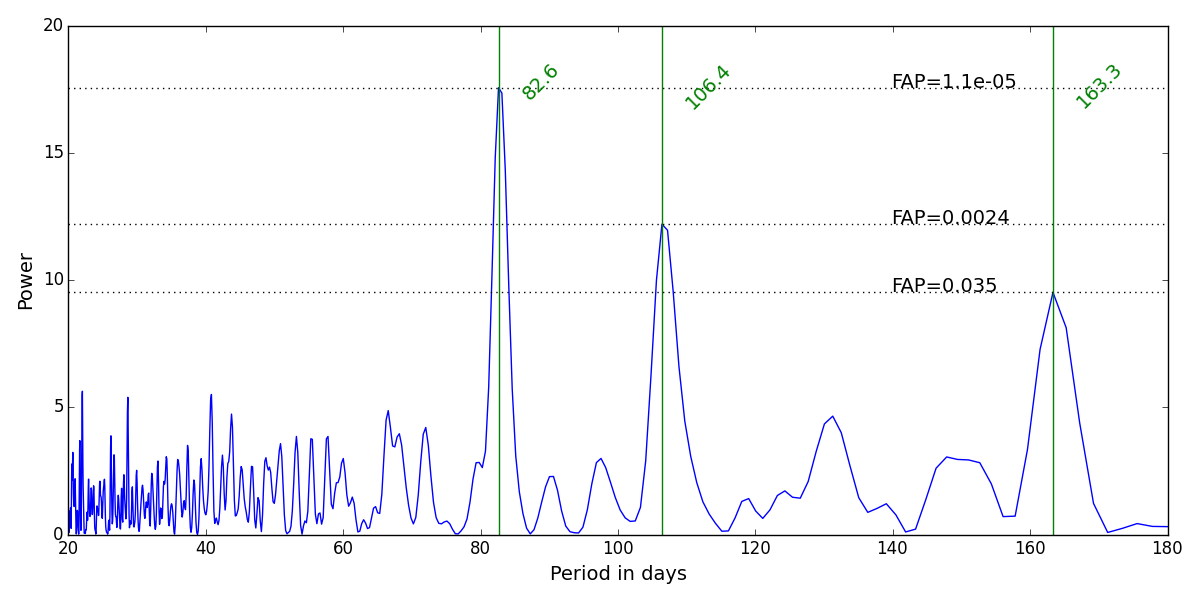
\includegraphics[scale=0.30]{Figures/asasnobin.png} \\
\end{center}
\caption{This is a periodogram from the {\asas} database for {\prox} second aperture, without binning, containing 970
  points, considering only periods between 20 and 160 days.}
\protect\label{fig:asaspgram1}
\end{figure}

\begin{figure}[!htbp]
\begin{center}
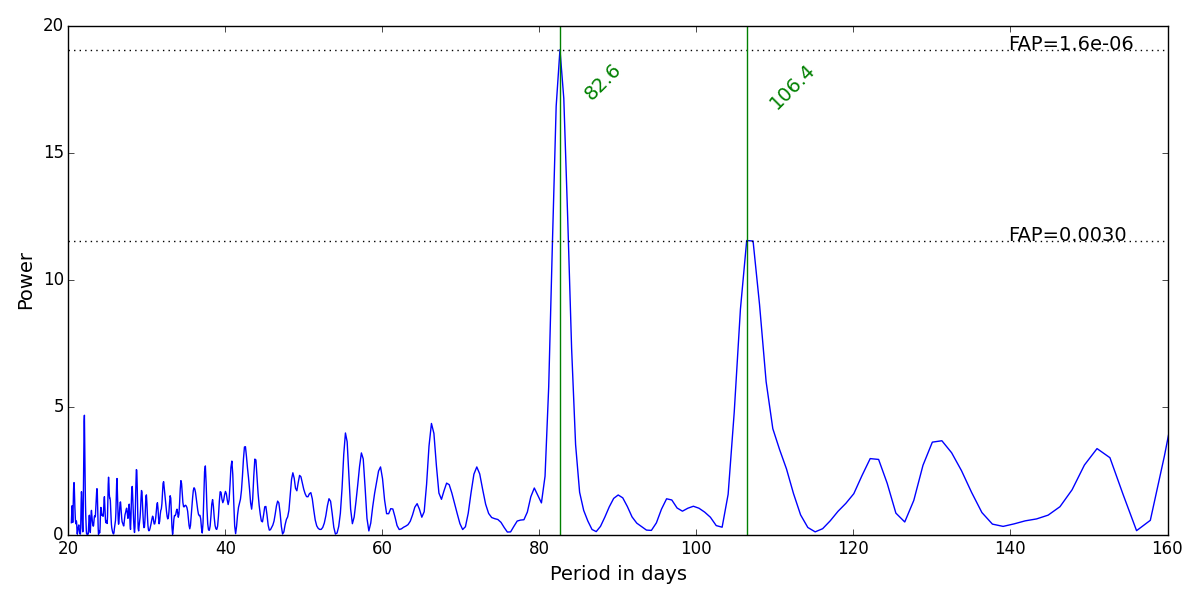
\includegraphics[scale=0.30]{Figures/asasbin1.png} \\
\end{center}
\caption{This is a periodogram from the {\asas} database for {\prox} second aperture, binned to 1 day, containing 624 points.}
\protect\label{fig:asaspgram2}
\end{figure}

\begin{figure}[!htbp]
\begin{center}
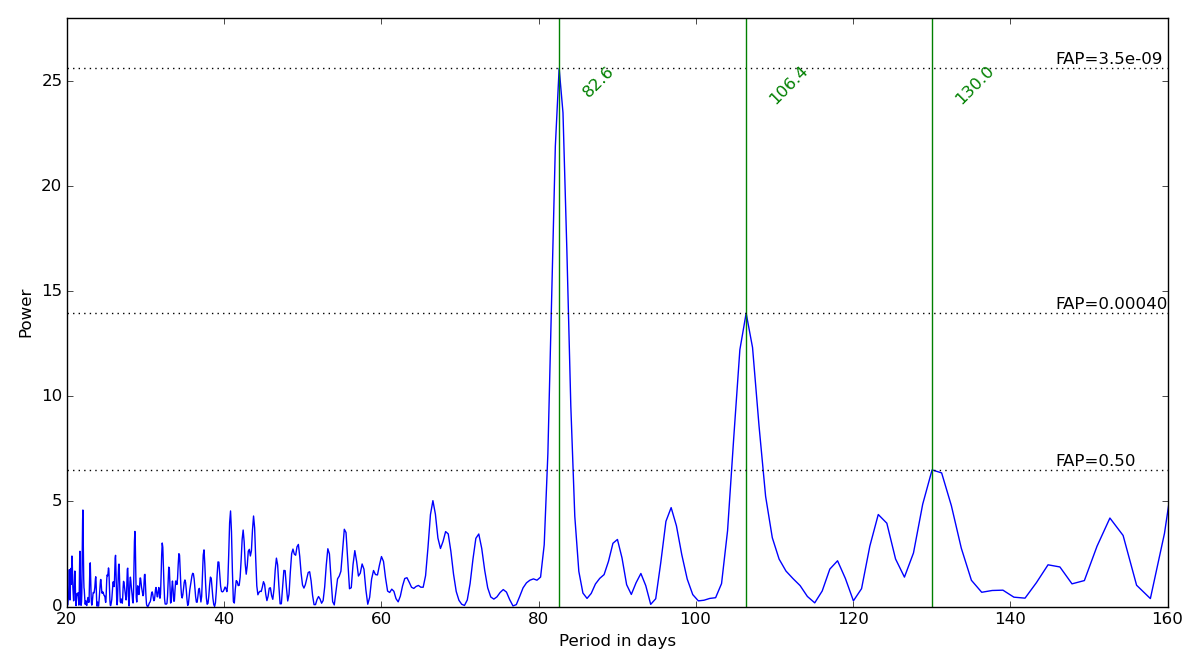
\includegraphics[scale=0.30]{Figures/asasbin18min.png} \\
\end{center}
\caption{This is a periodogram from the {\asas} database for {\prox} second aperture, binned to 18 minutes, containing 924 points.}
\protect\label{fig:asaspgram3}
\end{figure}

As some of the observations were duplicated or apparently overlapping, these were initially binned to 1 day, in line
with several of the {\harps} results described in section ??. This reduced the number of points to 624. From the result
the periodogram shown in Fig. \ref{fig:asaspgram2} was obtained. This appeared to clarify the peaks by reducing the
number with very short periods and enhancing the two major ones. Also attempted was the removal of clearly duplicated
points in the data, which could be done by binning to 18 minutes. This resulted in a more modest reduction to 924 points
and even smaller FAP of the main peak, to the order of $10^{-9}$. Also noticeable is that that the third highest peak is
in the region of 130 dayshas an FAP of 0.5.

Although the recommended aperture by {\asas} for {\prox} is the second aperture, it appeared valuable to compare the
three highest peaks from each of the apertures finding that nearly all the data gave a first peak of 82.6 days, a second
peak of 106.4 days and a much smaller third peak of about 131 days in most cases. The results are listed with
no-binning, 1-day and 18-minute binnings in Table \ref{table:asasperiods}. Also considered were the other grades of
{\asas} data, mostly from ID 142944-6241.0, with a little under half of the Class A Data, 416 points and much higher
error rating. All the periodograms from this lower quality data still showed a strong peak of around 82.5 days. The
results for 18-minute binning are shown in Table \ref{table:lqasas}.

\begin{table}[!htbp]
\centering
\scalebox{0.8}{
\begin{tabular}{|l|l|r|r|r|}
\hline
Aperture & binning & Peak 1 & Peak 2 & Peak 3 \\\hline
1 & none & 83.1 & 106.4 & 131.3 \\
2 & none & 82.6 & 106.4 & 22.0 \\
3 & none & 82.6 & 106.4 & 131.3 \\
4 & none & 82.6 & 106.4 & 131.3 \\
5 & none & 82.6 & 106.4 & 131.3 \\\hline
1 & 1 day & 82.6 & 106.4 & 110.6 \\
2 & 1 day & 82.6 & 106.4 & 22.0 \\
3 & 1 day & 82.6 & 106.4 & 130.0 \\
4 & 1 day & 82.6 & 106.4 & 42.6 \\
5 & 1 day & 82.6 & 106.4 & 42.4 \\\hline
1 & 18 min & 83.1 & 106.4 & 131.3 \\
2 & 18 min & 82.6 & 106.4 & 130.0 \\
3 & 18 min & 82.6 & 106.4 & 130.0 \\
4 & 18 min & 82.6 & 106.4 & 130.0 \\
5 & 18 min & 82.6 & 106.4 & 131.3 \\\hline
\end{tabular}}
\caption{Summary of three strongest periods taken from Class A values in {\asas} dataset for {\prox} from all apertures based upon magnitudes measured
  between December 2000 and September 2009. Results are shown for the raw data. 1-day binning and 18-minute binning.}
\protect\label{table:asasperiods}
\end{table}

\begin{table}[!htbp]
\centering
\scalebox{0.75}{
\begin{tabular}{|l|r|l|r|l|r|l|}
\hline
Aperture & Peak 1 & FAP & Peak 2 & FAP & Peak 3 & FAP \\\hline
1 & 83.1 & 0.0067 & 105.8 & 0.33 & 127.4 & 0.82 \\
2 & 83.1 & 0.03 & 105.8 & 0.43 & 127.4 & 0.61 \\
3 & 83.1 & 0.038 & 105.8 & 0.31 & 128.7 & 0.89 \\
4 & 84.1 & 0.1 & 105.8 & 0.21 & 128.7 & 0.93 \\
5 & 84.1 & 0.0024 & 105.8 & 0.0028 & 82.5 & 0.0033 \\\hline
\end{tabular}}
\caption{Summary of three strongest periods taken from Class B and lower quality values in {\asas} datasets for {\prox}
  based upon magnitudes measured between December 2000 and September 2009 binned to 18 minutes.}
\protect\label{table:lqasas}
\end{table}

It was noticeable that all of the Lomb-Scargle routines listed in Appendix \ref{chapter:lsroutines} gave exactly
the same results (apart from differences to scaling of the power) with all the {\asas} data, including the lower quality
data. This was in contrast to the Spectroscopic resutls discussed in later chapters of this \paperorthesis.

A search was made for very long periods up to the period spanned by the data in each case, however no strong periods
could be found, in particular nothing close to the 442 days reported in \citet{cincunegui07}.

\section{HST}
\protect\label{section:hst}

As another source of photometric results. periodograms were derived from the  {\hst} data discussed in
\citealt{benedict92,benedict98} consisting of 171 points obtained between July 1995 and January 1998, later enhanced so
the last 18 points extended to January 2001, Three times were actually duplicated and eliminating the duplications, it
was possible to obtain the periodogram in Fig. \ref{fig:hstb4min}.

\begin{figure}[!htbp]
\begin{center}
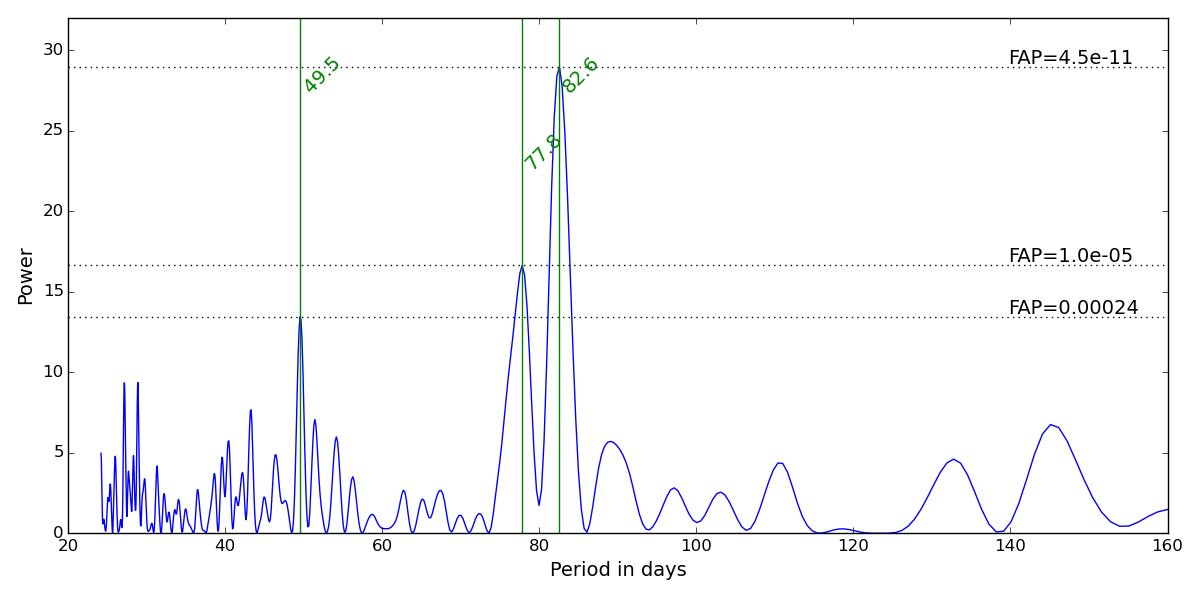
\includegraphics[scale=0.50]{Figures/hstb4min.png} \\
\end{center}
\caption{This is a periodogram from the {\hst} data discussed in \citet{benedict98} between July 1995 and January 1998 plus some additional
  points up to January 2001 examining periods showing the three highest peaks and with the FAPs marked in.}
\protect\label{fig:hstb4min}
\end{figure}

Again, as with the {\asas} data, all the Lomb-Scargle routines listed in Appendix \ref{chapter:lsroutines} gave exactly
the same results (other than the scaling of the power).

\section{Summary of photometric results}
\protect\label{section:summphotometric}

The period at 82.6 days is clearly as a strong, very low-FAP peak in both the {\asas} and {\hst} data. It is almost
certainly the rotation period of {\prox}, seemingly with a small error bar, although some investigations in Section
\ref{section:asasfap} were undertaken partly to investigate this.

It also provides a convenient benchmark for assessing the accuracy and reliability of the other, less clear
Spectroscopic methods investigated in Chapter \ref{chapter:proxima} based on the {\ha} line.

The {\asas} data, including the lesser quality data also included a strong peak at 106.4 days but this was not seen on
the {\hst} data. The former, however, has observation times much more constrained by the time of year and it is
noticeable that:

\begin{center}

$ \frac{1}{\frac{1}{82.6} - \frac{1}{365.25}} = 106.7 $

\end{center}

This suggests the possibility that this period is an alias thrown up by the observation times as indeed the strong
77.8-day period seen in the HST data is a similar alias. In Section ?? the interactions between competing periods are
considered further.